\documentclass[10pt,a4paper]{article}
\usepackage[utf8]{inputenc}
\usepackage{amsmath}
\usepackage{amsfonts}
\usepackage{amssymb}
\usepackage{ulem}
\usepackage{graphicx}
\author{GIMENEZ Florian}
\title{Compte Rendu TP1 Modélisation Identification et Commande}

\begin{document}
\normalem

\begin{titlepage}
	\begin{center}
	\textsc{\Large Compte Rendu Mise à Niveau Algorithmique}\\
	\textsc{GIMENEZ Florian - M1 EEEA}\\
	\end{center}

\end{titlepage}

\tableofcontents
\pagebreak

\section{Traveaux Pratique 1}

\subsection{Programme affichant "Bonjour"}
\subsubsection{Code}
	\begin{figure}[h]
	\begin{center}
	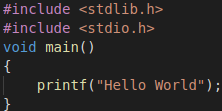
\includegraphics[scale=.4]{images/bonjour_c}
	\end{center}
	\caption{Programme C pour le programme Hello World}
	\end{figure}
\paragraph{}
    Pour afficher "Hello World" nous devons simplement placer un \emph{printf}.

\subsubsection{Résultat}
	\begin{figure}[h]
	\begin{center}
	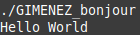
\includegraphics[scale=.4]{images/bonjour_ex}
	\end{center}
	\caption{Résultat du Programme \emph{bonjour}}
	\end{figure}

\subsection{Calcul Aire d'un disque}
\subsubsection{Code}
    \begin{figure}[h]
	\begin{center}
	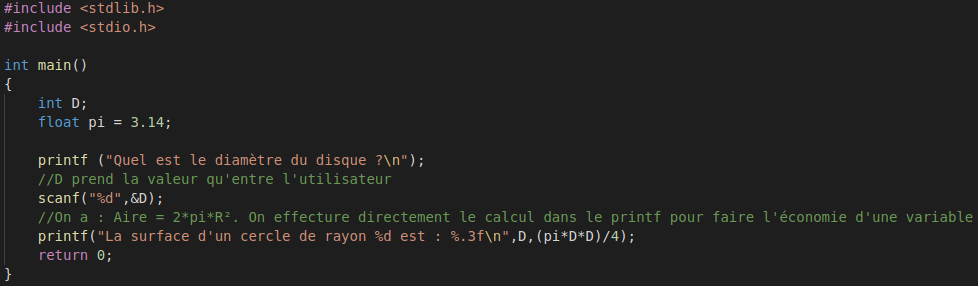
\includegraphics[scale=.3]{images/disque_c}
	\end{center}
	\caption{Programme C pour le calcul de l'aire d'un Disque}
	\end{figure}
\paragraph{}
Ici nous avons demandé le diamètre d'un disque pour pouvoir calculer son aire. Nous avons aussi affiché le résultat avec 3 
chiffres après la virgule. Nous avons aussi fait le calcul directement dans le \emph{printf}, pour faire l'économie d'une 
variable et rendre le programme plus lisible.
\pagebreak
\subsubsection{Résultat}
	\begin{figure}[h]
	\begin{center}
	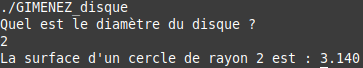
\includegraphics[scale=.3]{images/disque_ex}
	\end{center}
	\caption{Résultat du Programme \emph{disque}}
	\end{figure}


\subsection{Signe du produit}
\subsubsection{Code}
    \begin{figure}[h]
	\begin{center}
	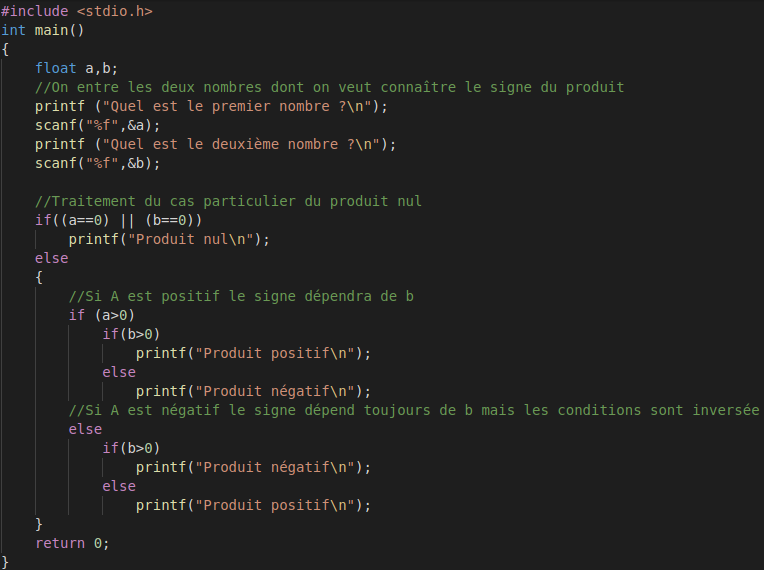
\includegraphics[scale=.3]{images/produit_c}
	\end{center}
	\caption{Programme C pour la déterminaion du signe d'un produit}
	\end{figure}
\paragraph{}
	Nous cherchons à determiner si le signe résultant du produit de deux nombres sera positif
	ou négatif. Pour cela nous testons tout d'abord le cas particulier où l'un des deux 
	nombre est nul. Par la suite en fonction du signe des nombres on pourra déterminer le signe 
	du résultat.
\subsubsection{Résultat}
	\begin{figure}[h]
	\begin{center}
	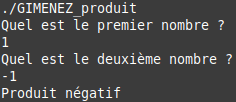
\includegraphics[scale=.3]{images/produit_ex}
	\end{center}
	\caption{Résultat du Programme \emph{produit}}
	\end{figure}

\pagebreak
\subsection{Polynôme}
\subsubsection{Code}
	\begin{figure}[h]
	\begin{center}
	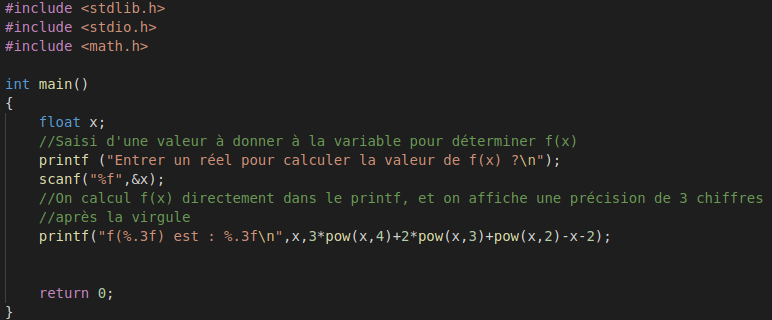
\includegraphics[scale=.3]{images/polynome_c}
	\end{center}
	\caption{Programme C pour le calcul d'une fonction}
	\end{figure}
\paragraph{}
	Nous souhaitons créer un programme permettant de calculer la valeur de la fonction 
	\emph{f} pour un \emph{x} donné. Nous avons utilisé la fonction \emph{power} de la librairie 
	math.h, pour effectuer les calculs de puissance.   
\subsubsection{Résultat}
	\begin{figure}[h]
	\begin{center}
	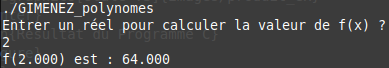
\includegraphics[scale=.3]{images/polynome_ex}
	\end{center}
	\caption{Résultat du Programme \emph{polynome}}
	\end{figure}

\pagebreak
\subsection{Conversion de secondes vers le format HH:MM:SS}
\subsubsection{Code}
	\begin{figure}[h]
	\begin{center}
	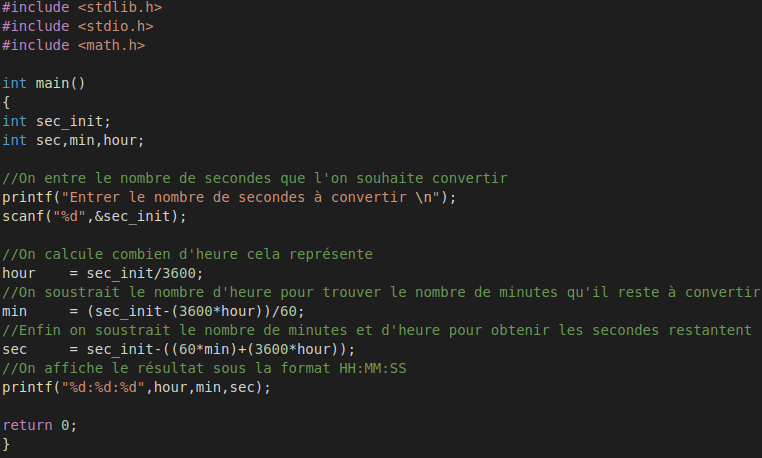
\includegraphics[scale=.3]{images/conversion_c}
	\end{center}
	\caption{Programme C pour la conversion d'un nombre de secondes en nombres d'heures, minutes et secondes}
	\end{figure}
\paragraph{}
	Nous avons ici créer un programme qui prend en entrées un nombre de secondes et qui l'a converti 
	en nombres d'heures, de minutes, et de secondes. On notera que pour ce programme toute les 
	divsions sont des divisions entière où on laisse le soin au compilateur d'arrondir les valeurs.
\subsubsection{Résultat}
	\begin{figure}[h]
	\begin{center}
	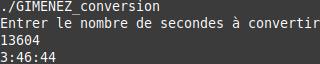
\includegraphics[scale=.3]{images/conversion_ex}
	\end{center}
	\caption{Résultat du Programme \emph{conversion}}
	\end{figure}

\pagebreak
\subsection{Calculatrice}
\subsubsection{Code}
	\begin{figure}[h]
	\begin{center}
	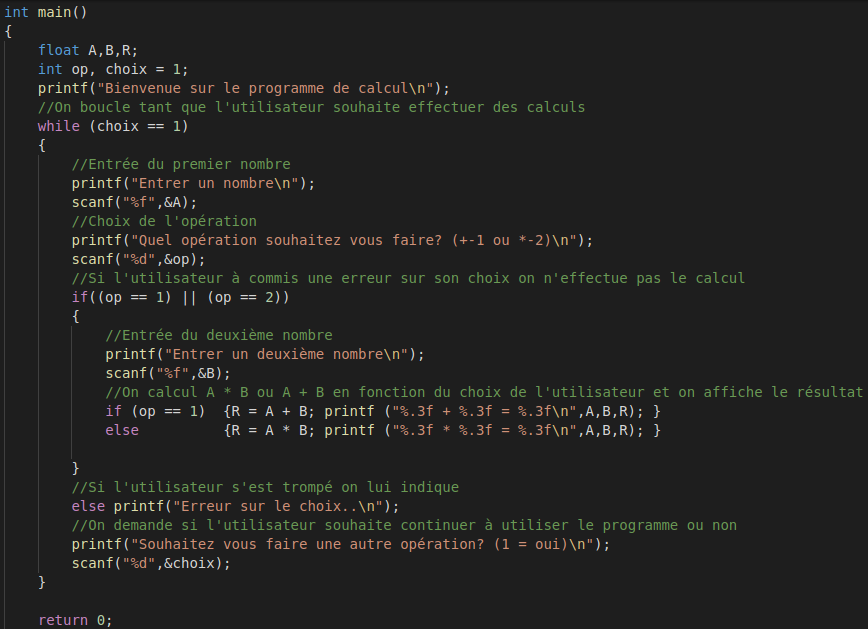
\includegraphics[scale=.3]{images/calculatrice_c}
	\end{center}
	\caption{Programme C pour la création d'une calculatrice}
	\end{figure}
\paragraph{}
	Ici nous avons créé un programme qui nous permet d'entrer deux nombres et d'effectuer une opération mathématique (+ ou *). 
	Nous demandons alors à l'utilisateur d'entrer un premier nombre puis un opération et enfin un deuxième nombre. On vérifie que 
	l'utilisateur à bien un opération valable.
	\pagebreak
\subsubsection{Résultat}
	\begin{figure}[h]
	\begin{center}
	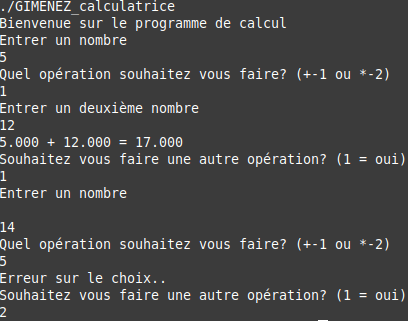
\includegraphics[scale=.3]{images/calculatrice_ex}
	\end{center}
	\caption{Résultat du Programme \emph{calculatrice}}
	\end{figure}

\section{Traveaux Pratique 2}

\subsection{Factorielle}
\subsubsection{Code}
	\begin{figure}[h]
	\begin{center}
	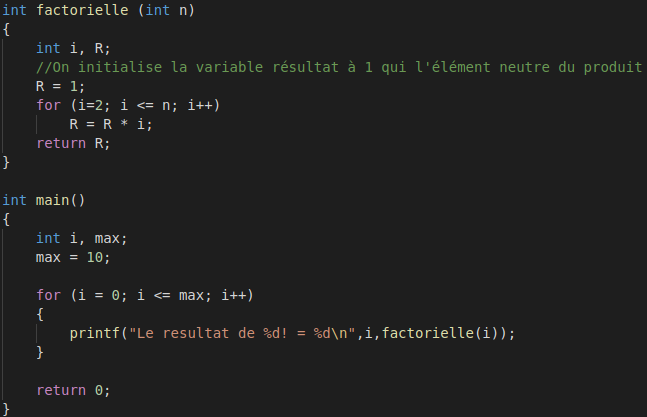
\includegraphics[scale=.3]{images/factorielle_c}
	\end{center}
	\caption{Programme C du calcul de la facotrielle}
	\end{figure}
\paragraph{}
	Le but de ce code était de pouvoir calculer la factorielle d'un nombre et aussi d'afficher les résultats intermédiaires. 
	On a ici créer une fonction pour faciliter la construction du texte. On a donc plus qu'a récupérer les valeurs et les afficher.
	La construction de la fonction fait que pour 0!, on obtient bien 1 comme résultat.
\pagebreak
\subsubsection{Résultat}
	\begin{figure}[h]
	\begin{center}
	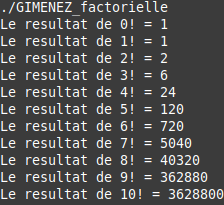
\includegraphics[scale=.3]{images/factorielle_ex}
	\end{center}
	\caption{Résultat du Programme \emph{factorielle}}
	\end{figure}


\subsection{Calcul de l'exponentiel}
\subsubsection{Approximation de e}
	\begin{figure}[h]
	\begin{center}
	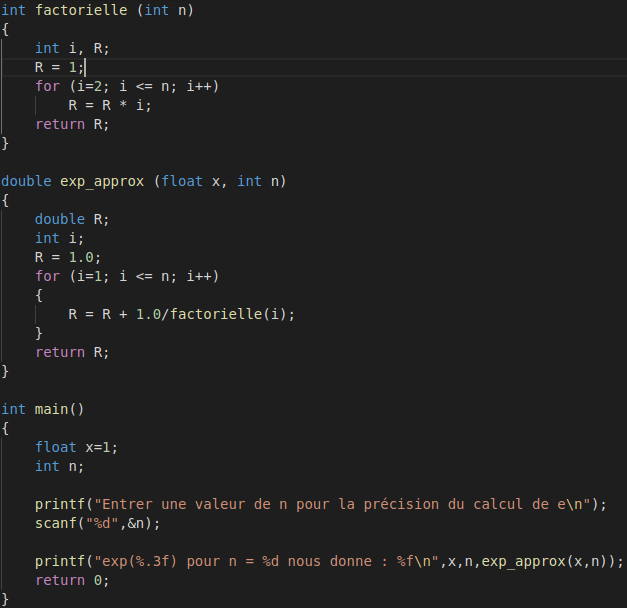
\includegraphics[scale=.3]{images/expo_1_c}
	\end{center}
	\caption{Programme C du calcul de e}
	\end{figure}
\paragraph{}
	On a ici créé un programme qui nous permet d'approximer la valeur de \emph{e} pour une précision \emph{n} donnée.
	\begin{figure}[h]
	\begin{center}
	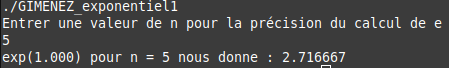
\includegraphics[scale=.3]{images/expo_1_ex}
	\end{center}
	\caption{Résultat du Programme pour \emph{n} = 5}
	\end{figure}

\subsubsection{Approximation de e, avec un condition sur la précision}
\begin{figure}[h]
\begin{center}
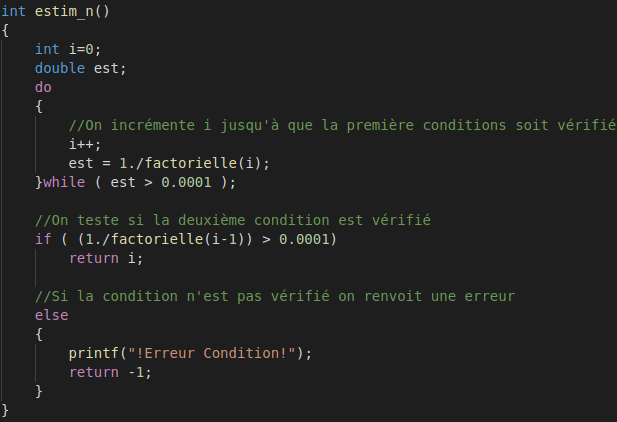
\includegraphics[scale=.3]{images/expo_2_c}
\end{center}
\caption{Programme C qui donne \emph{n} vérifiant notre condition}
\end{figure}
\paragraph{}
On souhaite maintenant créer un programme qui nous donnne un \emph{n} qui obéit aux la règles suivantes : 
$\frac{1}{(1-n)!} > 10^{-4}$ et $\frac{1}{n!} < 10^{-4}$ 
\begin{figure}[h]
\begin{center}
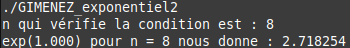
\includegraphics[scale=.3]{images/expo2_ex}
\end{center}
\caption{Résultat du Programme qui donne \emph{n} = 8}
\end{figure}

\subsection{Calcul de \emph{f(x)}}
\subsubsection{Code}
\begin{figure}[h]
\begin{center}
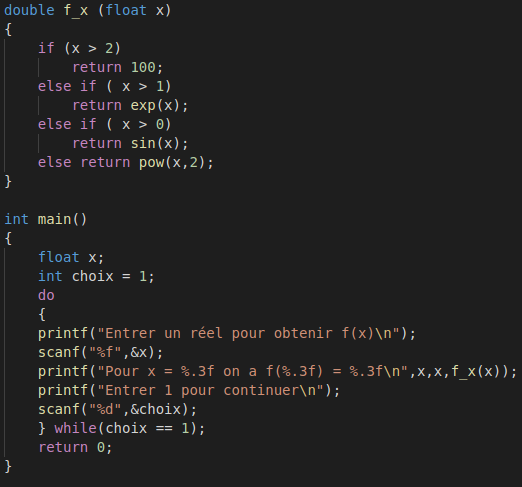
\includegraphics[scale=.3]{images/f_x_x}
\end{center}
\caption{Programme C définition de notre fonction \emph{f(x)}}
\end{figure}
\paragraph{}
On souhaite maintenant créer un programme qui nous donnne calcul l'image de la fonction f donnée. Pour cela nous 
avons défini chaque condition et renvoyons en fonction du \emph{x} donnée le résultat correspondant.
\subsubsection{Résultat}
\begin{figure}[h]
\begin{center}
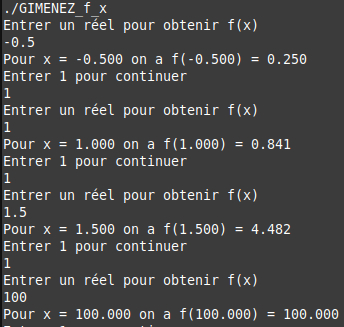
\includegraphics[scale=.3]{images/f_x_ex}
\end{center}
\caption{Résultat du Programme pour les x données dans l'énoncé}
\end{figure}
\pagebreak

\subsection{Inversion chiffres d'un nombre}
\subsubsection{Code}
\begin{figure}[h]
\begin{center}
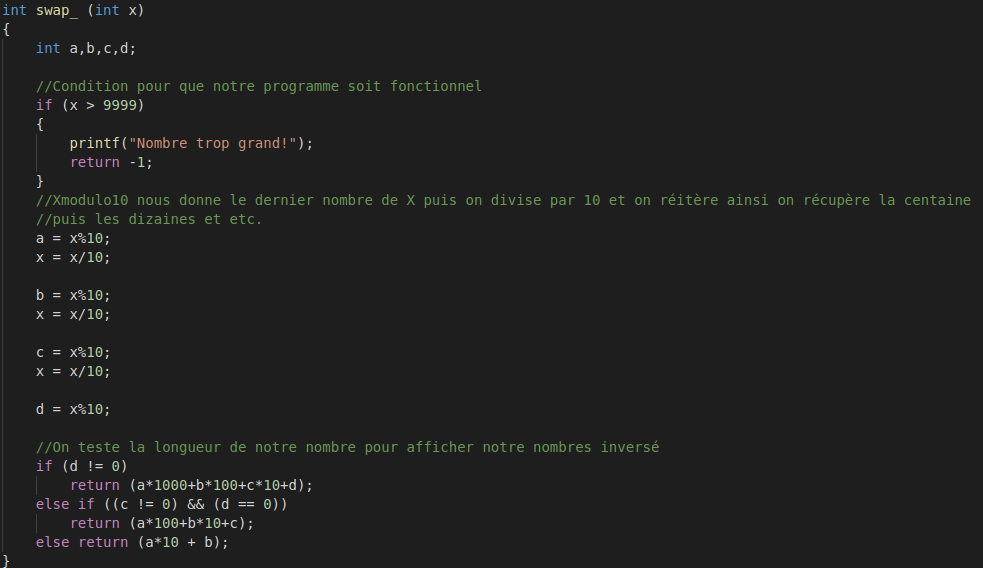
\includegraphics[scale=.3]{images/swap_c}
\end{center}
\caption{Programme C}
\end{figure}
\paragraph{}
On crée maintenant un programme permettant d'inverser l'entier entrer au clavier par l'utilisateur, 
par exemple si on prend le nombre 845, le programme doit nous renvoyer la valeur 548.
\subsubsection{Résultat}
\begin{figure}[h]
\begin{center}
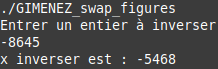
\includegraphics[scale=.3]{images/swap_ex}
\end{center}
\caption{Résultat du Programme avec un nombre négatif}
\end{figure}

\subsection{Calcul d'un nombre de visiteurs}
\subsubsection{Code}
\begin{figure}[h]
\begin{center}
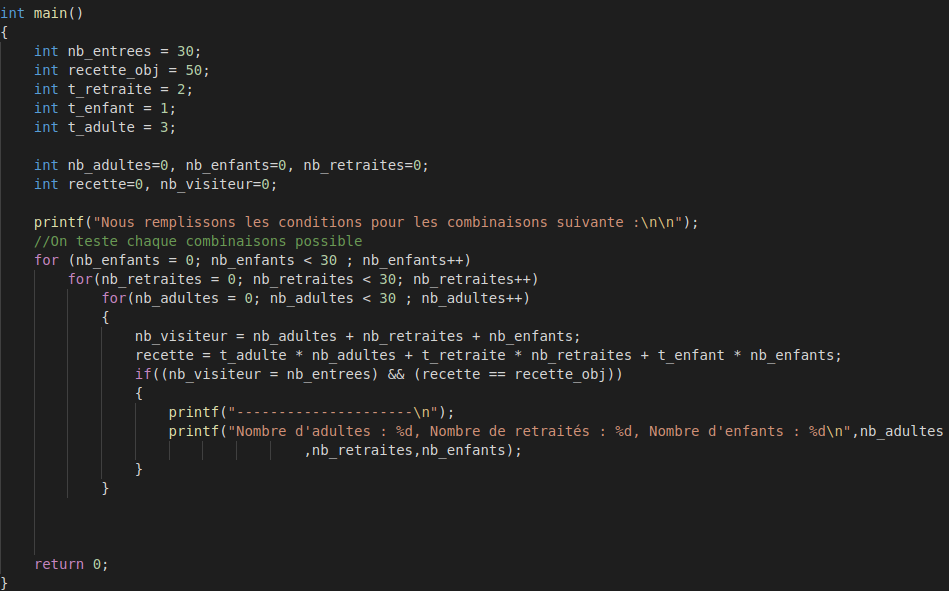
\includegraphics[scale=.3]{images/visiteurs_c}
\end{center}
\caption{Programme C}
\end{figure}
\paragraph{}
On souhaite connaitre toutes les possibilités de visiteurs qui respectent les conditions suivantes : \\
Le total des visiteurs d’un parc était de 30 personnes. Les tarifs appliqués sont
définis selon les catégories : 3 euros pour un adulte, 2 euros pour un retraité et 1 euros pour un enfant. La
recette des entrées était de 50 euros.
\subsubsection{Résultat}
\begin{figure}[h] 
\begin{center}
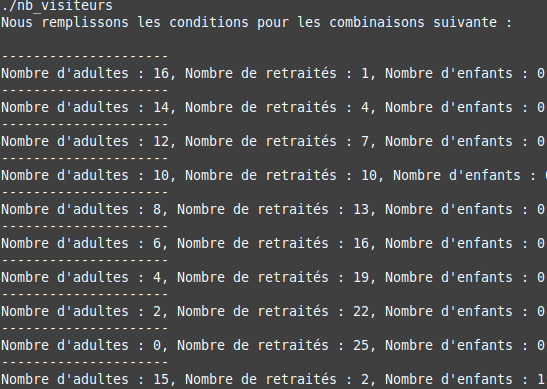
\includegraphics[scale=.3]{images/visit_ex_1}
\end{center}
\caption{Exemple de résultat}
\end{figure}
Ici nous avons trop de lignes résultats pour mettre en photo les voici donc ci dessous : \\
Nous remplissons les conditions pour les combinaisons suivantes :\\
\\
---------------------\\
Nombre d'adultes : 16, Nombre de retraités : 1, Nombre d'enfants : 0\\
---------------------\\
Nombre d'adultes : 14, Nombre de retraités : 4, Nombre d'enfants : 0\\
---------------------\\
Nombre d'adultes : 12, Nombre de retraités : 7, Nombre d'enfants : 0\\
---------------------\\
Nombre d'adultes : 10, Nombre de retraités : 10, Nombre d'enfants : 0\\
---------------------\\
Nombre d'adultes : 8, Nombre de retraités : 13, Nombre d'enfants : 0\\
---------------------\\
Nombre d'adultes : 6, Nombre de retraités : 16, Nombre d'enfants : 0\\
---------------------\\
Nombre d'adultes : 4, Nombre de retraités : 19, Nombre d'enfants : 0\\
---------------------\\
Nombre d'adultes : 2, Nombre de retraités : 22, Nombre d'enfants : 0\\
---------------------\\
Nombre d'adultes : 0, Nombre de retraités : 25, Nombre d'enfants : 0\\
---------------------\\
Nombre d'adultes : 15, Nombre de retraités : 2, Nombre d'enfants : 1\\
---------------------\\
Nombre d'adultes : 13, Nombre de retraités : 5, Nombre d'enfants : 1\\
---------------------\\
Nombre d'adultes : 11, Nombre de retraités : 8, Nombre d'enfants : 1\\
---------------------\\
Nombre d'adultes : 9, Nombre de retraités : 11, Nombre d'enfants : 1\\
---------------------\\
Nombre d'adultes : 7, Nombre de retraités : 14, Nombre d'enfants : 1\\
---------------------\\
Nombre d'adultes : 5, Nombre de retraités : 17, Nombre d'enfants : 1\\
---------------------\\
Nombre d'adultes : 3, Nombre de retraités : 20, Nombre d'enfants : 1\\
---------------------\\
Nombre d'adultes : 1, Nombre de retraités : 23, Nombre d'enfants : 1\\
---------------------\\
Nombre d'adultes : 16, Nombre de retraités : 0, Nombre d'enfants : 2\\
---------------------\\
Nombre d'adultes : 14, Nombre de retraités : 3, Nombre d'enfants : 2\\
---------------------\\
Nombre d'adultes : 12, Nombre de retraités : 6, Nombre d'enfants : 2\\
---------------------\\
Nombre d'adultes : 10, Nombre de retraités : 9, Nombre d'enfants : 2\\
---------------------\\
Nombre d'adultes : 8, Nombre de retraités : 12, Nombre d'enfants : 2\\
---------------------\\
Nombre d'adultes : 6, Nombre de retraités : 15, Nombre d'enfants : 2\\
---------------------\\
Nombre d'adultes : 4, Nombre de retraités : 18, Nombre d'enfants : 2\\
---------------------\\
Nombre d'adultes : 2, Nombre de retraités : 21, Nombre d'enfants : 2\\
---------------------\\
Nombre d'adultes : 0, Nombre de retraités : 24, Nombre d'enfants : 2\\
---------------------\\
Nombre d'adultes : 15, Nombre de retraités : 1, Nombre d'enfants : 3\\
---------------------\\
Nombre d'adultes : 13, Nombre de retraités : 4, Nombre d'enfants : 3\\
---------------------\\
Nombre d'adultes : 11, Nombre de retraités : 7, Nombre d'enfants : 3\\
---------------------\\
Nombre d'adultes : 9, Nombre de retraités : 10, Nombre d'enfants : 3\\
---------------------\\
Nombre d'adultes : 7, Nombre de retraités : 13, Nombre d'enfants : 3\\
---------------------\\
Nombre d'adultes : 5, Nombre de retraités : 16, Nombre d'enfants : 3\\
---------------------\\
Nombre d'adultes : 3, Nombre de retraités : 19, Nombre d'enfants : 3\\
---------------------\\
Nombre d'adultes : 1, Nombre de retraités : 22, Nombre d'enfants : 3\\
---------------------\\
Nombre d'adultes : 14, Nombre de retraités : 2, Nombre d'enfants : 4\\
---------------------\\
Nombre d'adultes : 12, Nombre de retraités : 5, Nombre d'enfants : 4\\
---------------------\\
Nombre d'adultes : 10, Nombre de retraités : 8, Nombre d'enfants : 4\\
---------------------\\
Nombre d'adultes : 8, Nombre de retraités : 11, Nombre d'enfants : 4\\
---------------------\\
Nombre d'adultes : 6, Nombre de retraités : 14, Nombre d'enfants : 4\\
---------------------\\
Nombre d'adultes : 4, Nombre de retraités : 17, Nombre d'enfants : 4\\
---------------------\\
Nombre d'adultes : 2, Nombre de retraités : 20, Nombre d'enfants : 4\\
---------------------\\
Nombre d'adultes : 0, Nombre de retraités : 23, Nombre d'enfants : 4\\
---------------------\\
Nombre d'adultes : 15, Nombre de retraités : 0, Nombre d'enfants : 5\\
---------------------\\
Nombre d'adultes : 13, Nombre de retraités : 3, Nombre d'enfants : 5\\
---------------------\\
Nombre d'adultes : 11, Nombre de retraités : 6, Nombre d'enfants : 5\\
---------------------\\
Nombre d'adultes : 9, Nombre de retraités : 9, Nombre d'enfants : 5\\
---------------------\\
Nombre d'adultes : 7, Nombre de retraités : 12, Nombre d'enfants : 5\\
---------------------\\
Nombre d'adultes : 5, Nombre de retraités : 15, Nombre d'enfants : 5\\
---------------------\\
Nombre d'adultes : 3, Nombre de retraités : 18, Nombre d'enfants : 5\\
---------------------\\
Nombre d'adultes : 1, Nombre de retraités : 21, Nombre d'enfants : 5\\
---------------------\\
Nombre d'adultes : 14, Nombre de retraités : 1, Nombre d'enfants : 6\\
---------------------\\
Nombre d'adultes : 12, Nombre de retraités : 4, Nombre d'enfants : 6\\
---------------------\\
Nombre d'adultes : 10, Nombre de retraités : 7, Nombre d'enfants : 6\\
---------------------\\
Nombre d'adultes : 8, Nombre de retraités : 10, Nombre d'enfants : 6\\
---------------------\\
Nombre d'adultes : 6, Nombre de retraités : 13, Nombre d'enfants : 6\\
---------------------\\
Nombre d'adultes : 4, Nombre de retraités : 16, Nombre d'enfants : 6\\
---------------------\\
Nombre d'adultes : 2, Nombre de retraités : 19, Nombre d'enfants : 6\\
---------------------\\
Nombre d'adultes : 0, Nombre de retraités : 22, Nombre d'enfants : 6\\
---------------------\\
Nombre d'adultes : 13, Nombre de retraités : 2, Nombre d'enfants : 7\\
---------------------\\
Nombre d'adultes : 11, Nombre de retraités : 5, Nombre d'enfants : 7\\
---------------------\\
Nombre d'adultes : 9, Nombre de retraités : 8, Nombre d'enfants : 7\\
---------------------\\
Nombre d'adultes : 7, Nombre de retraités : 11, Nombre d'enfants : 7\\
---------------------\\
Nombre d'adultes : 5, Nombre de retraités : 14, Nombre d'enfants : 7\\
---------------------\\
Nombre d'adultes : 3, Nombre de retraités : 17, Nombre d'enfants : 7\\
---------------------\\
Nombre d'adultes : 1, Nombre de retraités : 20, Nombre d'enfants : 7\\
---------------------\\
Nombre d'adultes : 14, Nombre de retraités : 0, Nombre d'enfants : 8\\
---------------------\\
Nombre d'adultes : 12, Nombre de retraités : 3, Nombre d'enfants : 8\\
---------------------\\
Nombre d'adultes : 10, Nombre de retraités : 6, Nombre d'enfants : 8\\
---------------------\\
Nombre d'adultes : 8, Nombre de retraités : 9, Nombre d'enfants : 8\\
---------------------\\
Nombre d'adultes : 6, Nombre de retraités : 12, Nombre d'enfants : 8\\
---------------------\\
Nombre d'adultes : 4, Nombre de retraités : 15, Nombre d'enfants : 8\\
---------------------\\
Nombre d'adultes : 2, Nombre de retraités : 18, Nombre d'enfants : 8\\
---------------------\\
Nombre d'adultes : 0, Nombre de retraités : 21, Nombre d'enfants : 8\\
---------------------\\
Nombre d'adultes : 13, Nombre de retraités : 1, Nombre d'enfants : 9\\
---------------------\\
Nombre d'adultes : 11, Nombre de retraités : 4, Nombre d'enfants : 9\\
---------------------\\
Nombre d'adultes : 9, Nombre de retraités : 7, Nombre d'enfants : 9\\
---------------------\\
Nombre d'adultes : 7, Nombre de retraités : 10, Nombre d'enfants : 9\\
---------------------\\
Nombre d'adultes : 5, Nombre de retraités : 13, Nombre d'enfants : 9\\
---------------------\\
Nombre d'adultes : 3, Nombre de retraités : 16, Nombre d'enfants : 9\\
---------------------\\
Nombre d'adultes : 1, Nombre de retraités : 19, Nombre d'enfants : 9\\
---------------------\\
Nombre d'adultes : 12, Nombre de retraités : 2, Nombre d'enfants : 10\\
---------------------\\
Nombre d'adultes : 10, Nombre de retraités : 5, Nombre d'enfants : 10\\
---------------------\\
Nombre d'adultes : 8, Nombre de retraités : 8, Nombre d'enfants : 10\\
---------------------\\
Nombre d'adultes : 6, Nombre de retraités : 11, Nombre d'enfants : 10\\
---------------------\\
Nombre d'adultes : 4, Nombre de retraités : 14, Nombre d'enfants : 10\\
---------------------\\
Nombre d'adultes : 2, Nombre de retraités : 17, Nombre d'enfants : 10\\
---------------------\\
Nombre d'adultes : 0, Nombre de retraités : 20, Nombre d'enfants : 10\\
---------------------\\
Nombre d'adultes : 13, Nombre de retraités : 0, Nombre d'enfants : 11\\
---------------------\\
Nombre d'adultes : 11, Nombre de retraités : 3, Nombre d'enfants : 11\\
---------------------\\
Nombre d'adultes : 9, Nombre de retraités : 6, Nombre d'enfants : 11\\
---------------------\\
Nombre d'adultes : 7, Nombre de retraités : 9, Nombre d'enfants : 11\\
---------------------\\
Nombre d'adultes : 5, Nombre de retraités : 12, Nombre d'enfants : 11\\
---------------------\\
Nombre d'adultes : 3, Nombre de retraités : 15, Nombre d'enfants : 11\\
---------------------\\
Nombre d'adultes : 1, Nombre de retraités : 18, Nombre d'enfants : 11\\
---------------------\\
Nombre d'adultes : 12, Nombre de retraités : 1, Nombre d'enfants : 12\\
---------------------\\
Nombre d'adultes : 10, Nombre de retraités : 4, Nombre d'enfants : 12\\
---------------------\\
Nombre d'adultes : 8, Nombre de retraités : 7, Nombre d'enfants : 12\\
---------------------\\
Nombre d'adultes : 6, Nombre de retraités : 10, Nombre d'enfants : 12\\
---------------------\\
Nombre d'adultes : 4, Nombre de retraités : 13, Nombre d'enfants : 12\\
---------------------\\
Nombre d'adultes : 2, Nombre de retraités : 16, Nombre d'enfants : 12\\
---------------------\\
Nombre d'adultes : 0, Nombre de retraités : 19, Nombre d'enfants : 12\\
---------------------\\
Nombre d'adultes : 11, Nombre de retraités : 2, Nombre d'enfants : 13\\
---------------------\\
Nombre d'adultes : 9, Nombre de retraités : 5, Nombre d'enfants : 13\\
---------------------\\
Nombre d'adultes : 7, Nombre de retraités : 8, Nombre d'enfants : 13\\
---------------------\\
Nombre d'adultes : 5, Nombre de retraités : 11, Nombre d'enfants : 13\\
---------------------\\
Nombre d'adultes : 3, Nombre de retraités : 14, Nombre d'enfants : 13\\
---------------------\\
Nombre d'adultes : 1, Nombre de retraités : 17, Nombre d'enfants : 13\\
---------------------\\
Nombre d'adultes : 12, Nombre de retraités : 0, Nombre d'enfants : 14\\
---------------------\\
Nombre d'adultes : 10, Nombre de retraités : 3, Nombre d'enfants : 14\\
---------------------\\
Nombre d'adultes : 8, Nombre de retraités : 6, Nombre d'enfants : 14\\
---------------------\\
Nombre d'adultes : 6, Nombre de retraités : 9, Nombre d'enfants : 14\\
---------------------\\
Nombre d'adultes : 4, Nombre de retraités : 12, Nombre d'enfants : 14\\
---------------------\\
Nombre d'adultes : 2, Nombre de retraités : 15, Nombre d'enfants : 14\\
---------------------\\
Nombre d'adultes : 0, Nombre de retraités : 18, Nombre d'enfants : 14\\
---------------------\\
Nombre d'adultes : 11, Nombre de retraités : 1, Nombre d'enfants : 15\\
---------------------\\
Nombre d'adultes : 9, Nombre de retraités : 4, Nombre d'enfants : 15\\
---------------------\\
Nombre d'adultes : 7, Nombre de retraités : 7, Nombre d'enfants : 15\\
---------------------\\
Nombre d'adultes : 5, Nombre de retraités : 10, Nombre d'enfants : 15\\
---------------------\\
Nombre d'adultes : 3, Nombre de retraités : 13, Nombre d'enfants : 15\\
---------------------\\
Nombre d'adultes : 1, Nombre de retraités : 16, Nombre d'enfants : 15\\
---------------------\\
Nombre d'adultes : 10, Nombre de retraités : 2, Nombre d'enfants : 16\\
---------------------\\
Nombre d'adultes : 8, Nombre de retraités : 5, Nombre d'enfants : 16\\
---------------------\\
Nombre d'adultes : 6, Nombre de retraités : 8, Nombre d'enfants : 16\\
---------------------\\
Nombre d'adultes : 4, Nombre de retraités : 11, Nombre d'enfants : 16\\
---------------------\\
Nombre d'adultes : 2, Nombre de retraités : 14, Nombre d'enfants : 16\\
---------------------\\
Nombre d'adultes : 0, Nombre de retraités : 17, Nombre d'enfants : 16\\
---------------------\\
Nombre d'adultes : 11, Nombre de retraités : 0, Nombre d'enfants : 17\\
---------------------\\
Nombre d'adultes : 9, Nombre de retraités : 3, Nombre d'enfants : 17\\
---------------------\\
Nombre d'adultes : 7, Nombre de retraités : 6, Nombre d'enfants : 17\\
---------------------\\
Nombre d'adultes : 5, Nombre de retraités : 9, Nombre d'enfants : 17\\
---------------------\\
Nombre d'adultes : 3, Nombre de retraités : 12, Nombre d'enfants : 17\\
---------------------\\
Nombre d'adultes : 1, Nombre de retraités : 15, Nombre d'enfants : 17\\
---------------------\\
Nombre d'adultes : 10, Nombre de retraités : 1, Nombre d'enfants : 18\\
---------------------\\
Nombre d'adultes : 8, Nombre de retraités : 4, Nombre d'enfants : 18\\
---------------------\\
Nombre d'adultes : 6, Nombre de retraités : 7, Nombre d'enfants : 18\\
---------------------\\
Nombre d'adultes : 4, Nombre de retraités : 10, Nombre d'enfants : 18\\
---------------------\\
Nombre d'adultes : 2, Nombre de retraités : 13, Nombre d'enfants : 18\\
---------------------\\
Nombre d'adultes : 0, Nombre de retraités : 16, Nombre d'enfants : 18\\
---------------------\\
Nombre d'adultes : 9, Nombre de retraités : 2, Nombre d'enfants : 19\\
---------------------\\
Nombre d'adultes : 7, Nombre de retraités : 5, Nombre d'enfants : 19\\
---------------------\\
Nombre d'adultes : 5, Nombre de retraités : 8, Nombre d'enfants : 19\\
---------------------\\
Nombre d'adultes : 3, Nombre de retraités : 11, Nombre d'enfants : 19\\
---------------------\\
Nombre d'adultes : 1, Nombre de retraités : 14, Nombre d'enfants : 19\\
---------------------\\
Nombre d'adultes : 10, Nombre de retraités : 0, Nombre d'enfants : 20\\
---------------------\\
Nombre d'adultes : 8, Nombre de retraités : 3, Nombre d'enfants : 20\\
---------------------\\
Nombre d'adultes : 6, Nombre de retraités : 6, Nombre d'enfants : 20\\
---------------------\\
Nombre d'adultes : 4, Nombre de retraités : 9, Nombre d'enfants : 20\\
---------------------\\
Nombre d'adultes : 2, Nombre de retraités : 12, Nombre d'enfants : 20\\
---------------------\\
Nombre d'adultes : 0, Nombre de retraités : 15, Nombre d'enfants : 20\\
---------------------\\
Nombre d'adultes : 9, Nombre de retraités : 1, Nombre d'enfants : 21\\
---------------------\\
Nombre d'adultes : 7, Nombre de retraités : 4, Nombre d'enfants : 21\\
---------------------\\
Nombre d'adultes : 5, Nombre de retraités : 7, Nombre d'enfants : 21\\
---------------------\\
Nombre d'adultes : 3, Nombre de retraités : 10, Nombre d'enfants : 21\\
---------------------\\
Nombre d'adultes : 1, Nombre de retraités : 13, Nombre d'enfants : 21\\
---------------------\\
Nombre d'adultes : 8, Nombre de retraités : 2, Nombre d'enfants : 22\\
---------------------\\
Nombre d'adultes : 6, Nombre de retraités : 5, Nombre d'enfants : 22\\
---------------------\\
Nombre d'adultes : 4, Nombre de retraités : 8, Nombre d'enfants : 22\\
---------------------\\
Nombre d'adultes : 2, Nombre de retraités : 11, Nombre d'enfants : 22\\
---------------------\\
Nombre d'adultes : 0, Nombre de retraités : 14, Nombre d'enfants : 22\\
---------------------\\
Nombre d'adultes : 9, Nombre de retraités : 0, Nombre d'enfants : 23\\
---------------------\\
Nombre d'adultes : 7, Nombre de retraités : 3, Nombre d'enfants : 23\\
---------------------\\
Nombre d'adultes : 5, Nombre de retraités : 6, Nombre d'enfants : 23\\
---------------------\\
Nombre d'adultes : 3, Nombre de retraités : 9, Nombre d'enfants : 23\\
---------------------\\
Nombre d'adultes : 1, Nombre de retraités : 12, Nombre d'enfants : 23\\
---------------------\\
Nombre d'adultes : 8, Nombre de retraités : 1, Nombre d'enfants : 24\\
---------------------\\
Nombre d'adultes : 6, Nombre de retraités : 4, Nombre d'enfants : 24\\
---------------------\\
Nombre d'adultes : 4, Nombre de retraités : 7, Nombre d'enfants : 24\\
---------------------\\
Nombre d'adultes : 2, Nombre de retraités : 10, Nombre d'enfants : 24\\
---------------------\\
Nombre d'adultes : 0, Nombre de retraités : 13, Nombre d'enfants : 24\\
---------------------\\
Nombre d'adultes : 7, Nombre de retraités : 2, Nombre d'enfants : 25\\
---------------------\\
Nombre d'adultes : 5, Nombre de retraités : 5, Nombre d'enfants : 25\\
---------------------\\
Nombre d'adultes : 3, Nombre de retraités : 8, Nombre d'enfants : 25\\
---------------------\\
Nombre d'adultes : 1, Nombre de retraités : 11, Nombre d'enfants : 25\\
---------------------\\
Nombre d'adultes : 8, Nombre de retraités : 0, Nombre d'enfants : 26\\
---------------------\\
Nombre d'adultes : 6, Nombre de retraités : 3, Nombre d'enfants : 26\\
---------------------\\
Nombre d'adultes : 4, Nombre de retraités : 6, Nombre d'enfants : 26\\
---------------------\\
Nombre d'adultes : 2, Nombre de retraités : 9, Nombre d'enfants : 26\\
---------------------\\
Nombre d'adultes : 0, Nombre de retraités : 12, Nombre d'enfants : 26\\
---------------------\\
Nombre d'adultes : 7, Nombre de retraités : 1, Nombre d'enfants : 27\\
---------------------\\
Nombre d'adultes : 5, Nombre de retraités : 4, Nombre d'enfants : 27\\
---------------------\\
Nombre d'adultes : 3, Nombre de retraités : 7, Nombre d'enfants : 27\\
---------------------\\
Nombre d'adultes : 1, Nombre de retraités : 10, Nombre d'enfants : 27\\
---------------------\\
Nombre d'adultes : 6, Nombre de retraités : 2, Nombre d'enfants : 28\\
---------------------\\
Nombre d'adultes : 4, Nombre de retraités : 5, Nombre d'enfants : 28\\
---------------------\\
Nombre d'adultes : 2, Nombre de retraités : 8, Nombre d'enfants : 28\\
---------------------\\
Nombre d'adultes : 0, Nombre de retraités : 11, Nombre d'enfants : 28\\
---------------------\\
Nombre d'adultes : 7, Nombre de retraités : 0, Nombre d'enfants : 29\\
---------------------\\
Nombre d'adultes : 5, Nombre de retraités : 3, Nombre d'enfants : 29\\
---------------------\\
Nombre d'adultes : 3, Nombre de retraités : 6, Nombre d'enfants : 29\\
---------------------\\
Nombre d'adultes : 1, Nombre de retraités : 9, Nombre d'enfants : 29\\ 

\pagebreak
\section{Traveaux Pratique 3}

\subsection{Etude d'un tableau}
\subsubsection{Code}
\begin{figure}[h]
\begin{center}
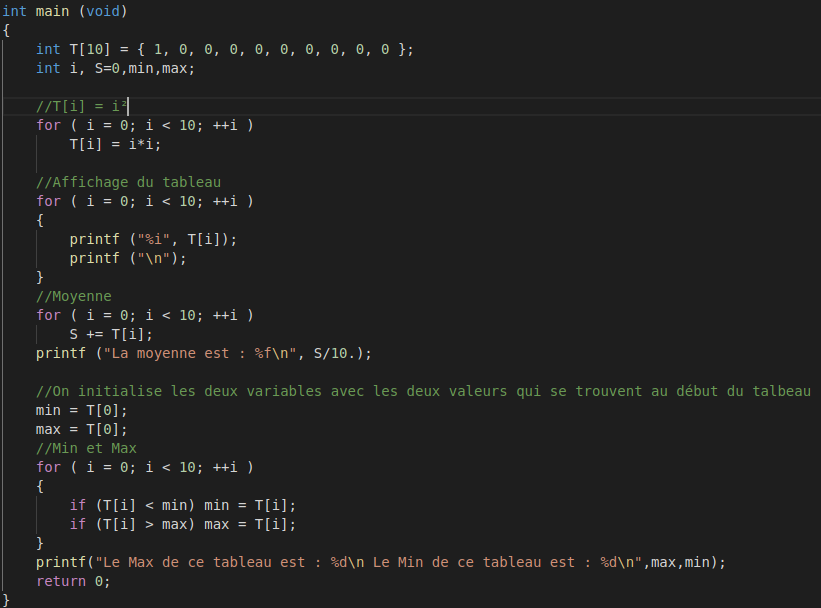
\includegraphics[scale=.3]{images/tab_1_c}
\end{center}
\caption{Programme C}
\end{figure}
\paragraph{}
Depuis le code nous avons ajouté le remplissage du tableau de tel sorte à avoir $T[i]=i^2$ sur l'ensemble de ce dernier. On a aussi 
implémenter la recherche du maximum, du minimum et de la moyenne.
\subsubsection{Résultat}
\begin{figure}[h] 
\begin{center}
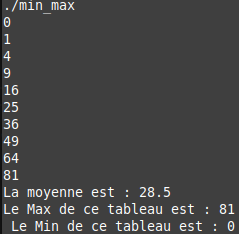
\includegraphics[scale=.3]{images/tab_1_ex}
\end{center}
\caption{Résultat}
\end{figure}



\subsection{Etude d'une Matrice}
\subsubsection{Code}
\begin{figure}[h]
\begin{center}
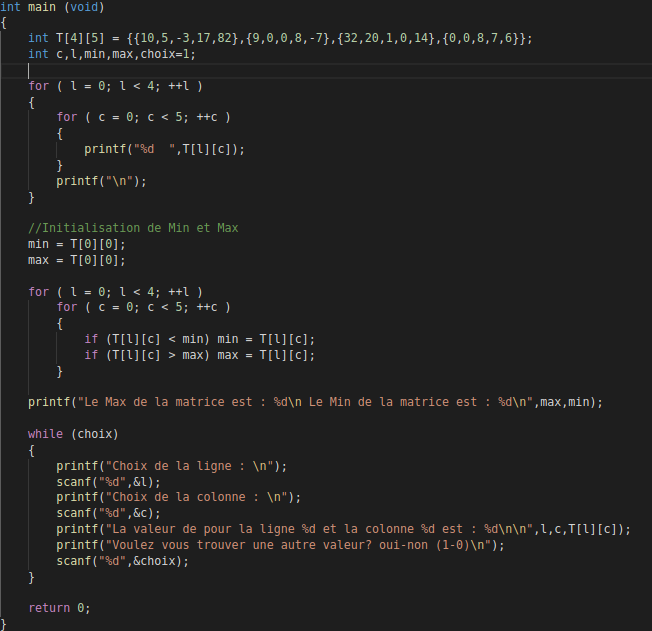
\includegraphics[scale=.3]{images/matrice_c}
\end{center}
\caption{Programme C}
\end{figure}
\paragraph{}
Ici nous avons entrer la matrice en dur dans le code puis chercher le minimum et le maximum et enfin par un jeu d'indice de tableau nous 
affichons les cases que l'utilisateur souhaite voir.
\subsubsection{Résultat}
\begin{figure}[h] 
\begin{center}
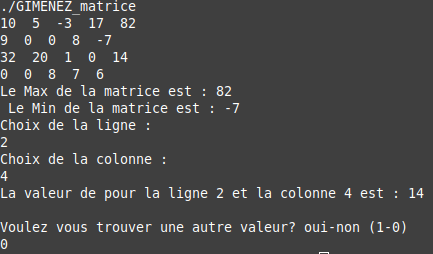
\includegraphics[scale=.3]{images/matrice_ex}
\end{center}
\caption{Résultat}
\end{figure}


\section{Traveaux Pratique 4}
\subsection{Exercice 1}
\subsubsection{Question 2}
\paragraph{}
Ici la variable p est un pointeur sur le tableau. Au premier printf, p nous donne la valeur de la première case. Lorsqu’on incrémente P on va pouvoir 
afficher les cases suivantes du tableaux.

\pagebreak	
\subsubsection{Question 3 : Affichage ordre croissant et décroissant}
\subsubsection{Code}
\begin{figure}[h]
\begin{center}
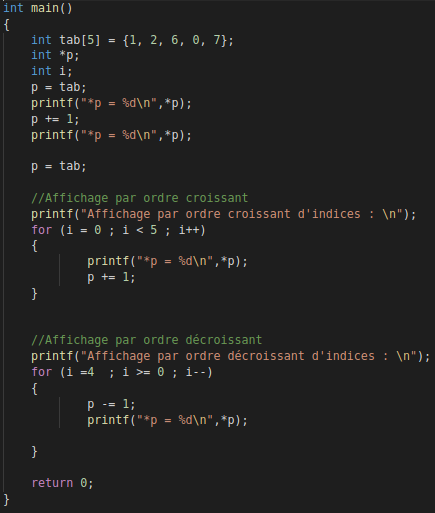
\includegraphics[scale=.3]{images/ex1_c}
\end{center}
\caption{Programme C}
\end{figure}
\paragraph{}
On applique ce que nous a appris la question précédente pour obtenir l'affichage du tableau dans l'ordre croissant 
des indices puis décroissant.
\subsubsection{Résultat}
\begin{figure}[h] 
\begin{center}
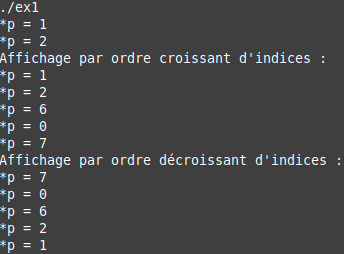
\includegraphics[scale=.3]{images/ex1_ex}
\end{center}
\caption{Résultat}
\end{figure}


\pagebreak
\subsection{Exercice 2}
\subsubsection{Code}
\begin{figure}[h]
	\begin{center}
	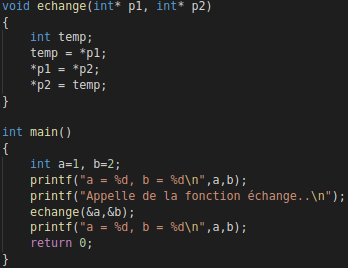
\includegraphics[scale=.3]{images/swap_p_c}
	\end{center}
	\caption{Programme C}
	\end{figure}
	\paragraph{}
	On utilise ici les propriétées propres aux pointeurs pour permettre un échange de valeurs entre deux variables.
	\subsubsection{Résultat}
	\begin{figure}[h] 
	\begin{center}
	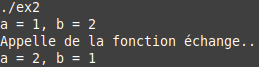
\includegraphics[scale=.3]{images/swap_p_ex}
	\end{center}
	\caption{Résultat}
	\end{figure}

\pagebreak
\subsection{Exercice 3}
\subsubsection{Code}
\begin{figure}[h]
\begin{center}
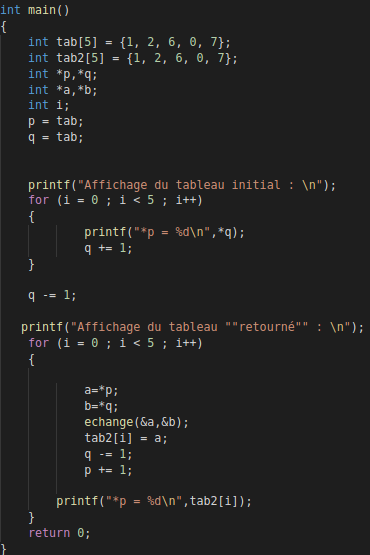
\includegraphics[scale=.3]{images/ex3_c}
\end{center}
\caption{Programme C}
\end{figure}
\paragraph{}
Ici nous utilisons la fonction défini précédemment pour inverser le tableau.
\subsubsection{Résultat}
\begin{figure}[h] 
\begin{center}
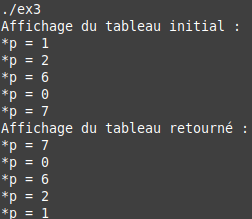
\includegraphics[scale=.3]{images/ex3_ex}
\end{center}
\caption{Résultat}
\end{figure}

\pagebreak
\subsection{Exercice 4}
\subsubsection{Code}
\begin{figure}[h]
\begin{center}
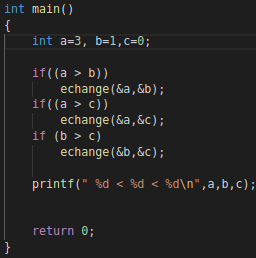
\includegraphics[scale=.3]{images/ex4_c}
\end{center}
\caption{Programme C}
\end{figure}
\paragraph{}
Ici nous utilisons la fonction défini précédemment pour échanger les valeurs jusqu'à que les valeurs soient trié par ordre croissant.
\subsubsection{Résultat}
\begin{figure}[h] 
\begin{center}
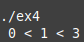
\includegraphics[scale=.3]{images/ex4_ex}
\end{center}
\caption{Résultat}
\end{figure}


\end{document}